\section{Transformation Rules}

\begin{center}
    {\Large\scshape Vertical Shift Up/Down}\\[0.5em]
    \renewcommand{\arraystretch}{1.5}
    \begin{tabular}{ r | c | c }
        \toprule
        \multirow{3}{*}{\Large   $g(x) = f(x) + k$   } 
            & {\large $g(x) = \myRoot{x} + 3$ }
            & {\large $g(x) = \myRoot{x} - 2$ }\\ \cline{2-3}
            %
            & $k=3$ 
            & $k=-2$ \\ \cline{2-3}
            %
            & shift up by 3 
            & shift down by 2 \\ 
        \bottomrule
    \end{tabular}
\end{center}

\begin{center}
    {\Large\scshape Horizontal Shift Left/Right} \\
    {\small $h$ is the {\itshape opposite} of what you see}\\[0.5em]
    \renewcommand{\arraystretch}{1.5}
    \begin{tabular}{ r | c | c }
        \toprule
        \multirow{3}{*}{\Large   $g(x) = f(x-h) $   } 
            & {\large $g(x) = \myRoot{x-5} $ } 
            & {\large $g(x) = \myRoot{x+1} $ } \\ \cline{2-3}
            %
            & $h=5$ 
            & $h=-1$ \\ \cline{2-3}
            %
            & shift right by 5 
            & shift left by 1 \\ 
        \bottomrule
    \end{tabular}
\end{center}

\begin{center}
    {\Large\scshape Vertical Stretch/Compression}\nopagebreak\\[0.5em]
    \renewcommand{\arraystretch}{1.5}
    \begin{tabular}{ r | l | l }
        \toprule
        \multirow{4}{*}{   \Large $g(x) = a f(x) $   } 
            & {\large $g(x) = 2 \myRoot{x} $ }
            & {\large $g(x) = \frac{1}{2} \myRoot{x} $} \\ \cline{2-3}
            %
            & $a=2$ 
            & $a=1/2$ \\ 
            %
            & {\small stretch when $a>1$}
            & {\small compression when $0<a<1$} \\ \cline{2-3}
            %
            & stretch by a factor of 5 
            & compress by a factor of $1/2$ \\ 
        \bottomrule
    \end{tabular}
\end{center}


\begin{center}
    {\Large\scshape Reflection Across the $x$-axis}\nopagebreak\\[0.5em]
    \renewcommand{\arraystretch}{1.5}
    \begin{tabular}{ r | l }
        \toprule
        \multirow{3}{*}{   \Large $g(x) = - f(x) $   } 
            & {\large $g(x) = - \myRoot{x} $ }  \\ \cline{2-2}
            & $a=-1$  \\ \cline{2-2}
            & 
            {
                \begin{tikzpicture}[
                    scale=0.25,
                    xaxe style/.style = { very thick, arrows={-{Straight Barb}}, label={}, },                 
                    yaxe style/.style = { very thick, arrows={-{Straight Barb}}, label={}, },                 
                ]
                \scriptsize
                \tkzInit[ xmax=6, xmin=-6,  ymax=6, ymin=-6, ]
                \tkzGrid
                \tkzDrawXY[label={},color=black,]
                % \tkzLabelX[orig=false,]
                % \tkzLabelY[orig=false,]
                \tkzFct[domain = 0:6,thick, solid]{sqrt(x)}
                \tkzText[right](5.8,2){\large $f$}
                %
                \tkzFct[domain = -6:6, thick, dashed]{-sqrt(x)}
                \tkzText[right](5.8,-2.5){\large$g$}
            \end{tikzpicture}
            } \\
        \bottomrule
    \end{tabular}
\end{center}
